\chapter{Diseño e implementación} % Main chapter title

En este capítulo se describe la arquitectura en detalle de la solución. Se presenta una breve introducción a los patrones de software utilizados con especial foco en las técnicas de concurrencia. El trabajo realizado utiliza la plataforma de hardware EDU-CIAA, la API desarrollada bajo el nombre de Firmware\_ v3, y el sistema operativo de tiempo real FreeRTOS.\\

Siguiendo los lineamientos del marco de trabajo en ingeniería de software, se presenta el siguiente orden: requerimientos, funcionalidades y casos de uso principales como ejes del espacio problema; arquitectura, patrones, firmware y hardware para describir el espacio solución.\\


\label{Chapter3} % Change X to a consecutive number; for referencing this chapter elsewhere, use \ref{ChapterX}

\definecolor{mygreen}{rgb}{0,0.6,0}
\definecolor{mygray}{rgb}{0.9,0.9,0.9}
\definecolor{mymauve}{rgb}{0.58,0,0.82}

%%%%%%%%%%%%%%%%%%%%%%%%%%%%%%%%%%%%%%%%%%%%%%%%%%%%%%%%%%%%%%%%%%%%%%%%%%%%%
% parámetros para configurar el formato del código en los entornos lstlisting
%%%%%%%%%%%%%%%%%%%%%%%%%%%%%%%%%%%%%%%%%%%%%%%%%%%%%%%%%%%%%%%%%%%%%%%%%%%%%
\lstset{ %
  backgroundcolor=\color{mygray},   % choose the background color; you must add \usepackage{color} or \usepackage{xcolor}
  basicstyle=\footnotesize,        % the size of the fonts that are used for the code
  breakatwhitespace=false,         % sets if automatic breaks should only happen at whitespace
  breaklines=true,                 % sets automatic line breaking
  captionpos=b,                    % sets the caption-position to bottom
  commentstyle=\color{mygreen},    % comment style
  deletekeywords={...},            % if you want to delete keywords from the given language
  %escapeinside={\%*}{*)},          % if you want to add LaTeX within your code
  %extendedchars=true,              % lets you use non-ASCII characters; for 8-bits encodings only, does not work with UTF-8
  %frame=single,	                % adds a frame around the code
  keepspaces=true,                 % keeps spaces in text, useful for keeping indentation of code (possibly needs columns=flexible)
  keywordstyle=\color{blue},       % keyword style
  language=[ANSI]C,                % the language of the code
  %otherkeywords={*,...},           % if you want to add more keywords to the set
  numbers=left,                    % where to put the line-numbers; possible values are (none, left, right)
  numbersep=5pt,                   % how far the line-numbers are from the code
  numberstyle=\tiny\color{mygray}, % the style that is used for the line-numbers
  rulecolor=\color{black},         % if not set, the frame-color may be changed on line-breaks within not-black text (e.g. comments (green here))
  showspaces=false,                % show spaces everywhere adding particular underscores; it overrides 'showstringspaces'
  showstringspaces=false,          % underline spaces within strings only
  showtabs=false,                  % show tabs within strings adding particular underscores
  stepnumber=1,                    % the step between two line-numbers. If it's 1, each line will be numbered
  stringstyle=\color{mymauve},     % string literal style
  tabsize=2,	                   % sets default tabsize to 2 spaces
  title=\lstname,                  % show the filename of files included with \lstinputlisting; also try caption instead of title
  morecomment=[s]{/*}{*/}
}
\lstdefinestyle{nonumbers}
{numbers=none}


A modo de ejemplo:

\begin{lstlisting}[
	language=C, 
	backgroundcolor=\color{mygray},
	style=nonumbers]

sStateMachine fsmTest [] = 
{
	{STATE_INIT, evInit, InitHandler},
	{STATE_LISTENING, evReceive, ListeningHandler},
	{STATE_HEADER, evReceive, HeaderHandler},
	{STATE_TRAILER, evReceive, TrailerHandler}
};
\end{lstlisting}
    


\section{Requerimientos}

\pagebreak
\section{Casos de Uso}

\pagebreak

\section{Arquitectura}

\subsection{Contexto}
\begin{figure}[ht]
	\centering
	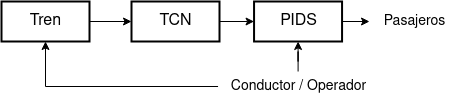
\includegraphics[width=1\textwidth]{./Figures/diagTrenTcnPids.png}
	\caption{Diagrama del sistema Tren-TCN-PIDS.}
	\label{fig:diagTrenTcnPids}
\end{figure}

\begin{figure}[ht]
	\centering
	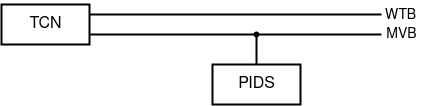
\includegraphics[width=1\textwidth]{./Figures/diagTcnPidsBusesWtbMvb.png}
	\caption{Diagrama de interconexión TCN-PIDS}
	\label{fig:diagTcnPidsBuusesWtbMvb}
\end{figure}


\begin{figure}[ht]
	\centering
	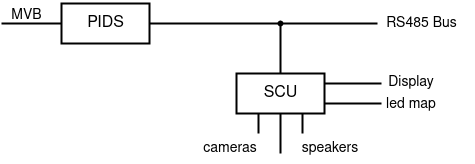
\includegraphics[width=1\textwidth]{./Figures/diagPidsScuDevices.png}
	\caption{Diagrama del módulo SCU en la red PIDS.}
	\label{fig:diagPidsScuDevices}
\end{figure}

\begin{figure}[ht]
	\centering
	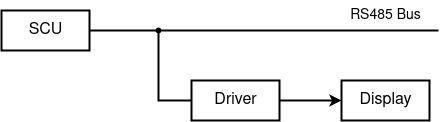
\includegraphics[width=1\textwidth]{./Figures/diagScuDriverDisplay.png}
	\caption{Diagrama de bloques del sistema SCU, placa de control y carteles LED de salón.}
	\label{fig:diagScuDriverDisplay}
\end{figure}

\pagebreak
\subsection{Diseño}


\begin{figure}[ht]
	\centering
	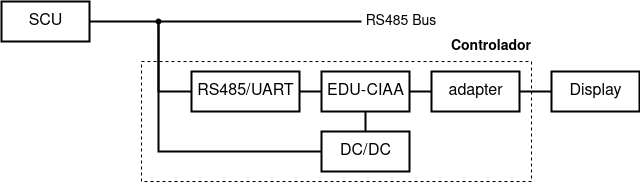
\includegraphics[width=1\textwidth]{./Figures/diagVistaReDisenhoEduCIAA.png}
	\caption{Diagrama de bloques del controlador propuesto.}
	\label{fig:diagVistaReDisenhoEduCIAA}
\end{figure}


\begin{figure}[ht]
	\centering
	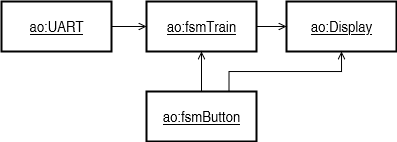
\includegraphics[width=1\textwidth]{./Figures/diagVistaDisenho.png}
	\caption{Vista de interacciones del sistema propuesto.}
	\label{fig:diagVistaDisenho}
\end{figure}

\begin{figure}[ht]
	\centering
	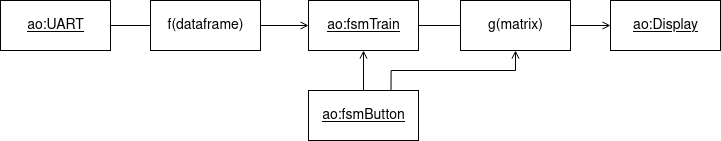
\includegraphics[width=1\textwidth]{./Figures/diagVistaDisenhoExtendida.png}
	\caption{Vista de interacciones extendida del sistema propuesto.}
	\label{fig:diagVistaDisenhoExtendida}
\end{figure}

\pagebreak
\subsection{Implementación}

El desarrollo de la arquitectura propuesta se basa en la interacción de máquinas de estado.
En este trabajo las máquinas de estado se implementan en C a partir de la siguiente estructura:

1. Definir los estados posibles con un tipo definido como "eSystemState":

\begin{lstlisting}[
	language=C, 
	backgroundcolor=\color{mygray},
	style=nonumbers]
typedef enum {
	STATE_INIT,
	STATE_LISTENING,
	STATE_HEADER,
	STATE_TRAILER
} eSystemState;
\end{lstlisting}

2. Definir los eventos que van a generar transiciones entre estados con un tipo definido "eSystemEvent":

\begin{lstlisting}[
	language=C, 
	backgroundcolor=\color{mygray},
	style=nonumbers]
typedef enum{
	evInit,
	evReceive,
	evHeader,
	evTrailer
} eSystemEvent;
\end{lstlisting}

3. A partir de un diagrama de la máquina de estados en cuestión, 
definir un tipo puntero a función definido como "*pfEventHandler()":

\begin{lstlisting}[
	language=C, 
	backgroundcolor=\color{mygray},
	style=nonumbers]
typedef eSystemState (*pfEventHandler)(void);
\end{lstlisting}

4: Definir una estructura para la máquina de estados con un tipo definido "sStateMachine" que incluya una variable estado (eSystemState), una variable evento (eSystemEvent) y un puntero a función (pfEventHandler). El puntero a función será una instancia de handler específico que maneje las transiciones entre estados. 

\begin{lstlisting}[
	language=C, 
	backgroundcolor=\color{mygray},
	style=nonumbers]
typedef struct{
	eSystemState 		fsmState;
	eSystemEvent 		fsmEvent;
	pfEventHandler 		fsmHandler;
} sStateMachine;
\end{lstlisting}

De esta manera queda desacoplada la implentación de los handlers del resto de la estructura de la máquina de estados, logrando portabilidad, escala y modularidad. Los handlers serán funciones que se implementan con el sufico Handler() y que por definición tienen un solo argumento de tipo void.

5. Definir los handlers a implementar para el manejo de ejecución y transiciones entre estados.

\begin{lstlisting}[
	language=C, 
	backgroundcolor=\color{mygray},
	style=nonumbers]

eSystemState 	InitHandler(void)		;
eSystemState 	ListeningHandler(void)	;
eSystemState 	HeaderHandler(void)		;
eSystemState 	TrailerHandler(void) 	;

\end{lstlisting}

Con esta técnica de desacoplamiento, se implementan dos archivos por cada máquina de estado : uno de encabezados (stateMachine.h) con las definiciones de los puntos 1 a 4 y otro con la implementación (stateMachine.c) de los handlers.

Una implementación de handler a modo de ejemplo se presenta a continuación.

\begin{lstlisting}[
	language=C, 
	backgroundcolor=\color{mygray},
	style=nonumbers]
eSystemState 	TrailerHandler(void){ 
	printf("STATE_TRAILER;\n");
	return STATE_LISTENING; 
}
\end{lstlisting}

6. Finalmente, cada implementación de máquina de estado debe definir la instancia de la máquina de estados propiamente dicha con un arreglo de estructuras definido como "sStateMachine fsmStateMachine []". Este arreglo de estructuras máquina de estados se define a partir de los estados, sus transiciones y los handlers correspondientes. En este punto es mandatorio incluir un diagrama de la máquina de estados.

\begin{lstlisting}[
	language=C, 
	backgroundcolor=\color{mygray},
	style=nonumbers]

sStateMachine fsmTest [] = 
{
	{STATE_INIT, evInit, InitHandler},
	{STATE_LISTENING, evReceive, ListeningHandler},
	{STATE_HEADER, evReceive, HeaderHandler},
	{STATE_TRAILER, evReceive, TrailerHandler}
};
\end{lstlisting}


El diagrama para esta máquina es el siguiente:

\begin{lstlisting}[
	language=C, 
	backgroundcolor=\color{mygray},
	style=nonumbers]
\end{lstlisting}


\begin{figure}[ht]
	\centering
	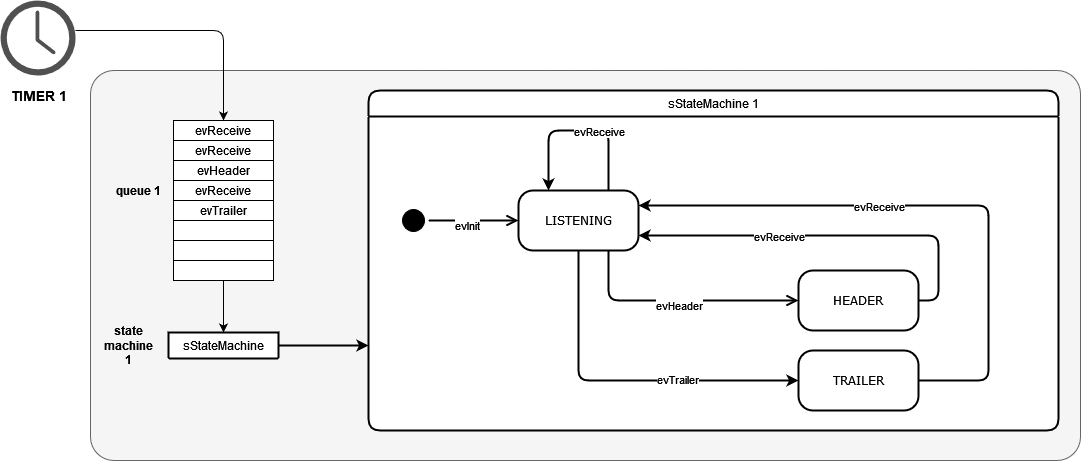
\includegraphics[width=1\textwidth]{./Figures/stateMachineUARTv1.png}
	\caption{Diagrama del objeto activo de la máquina de estados asociada.}
	\label{fig:fsmUARTv1}
\end{figure}

	
\pagebreak
\section{Patrones}



\begin{figure}[ht]
	\centering
	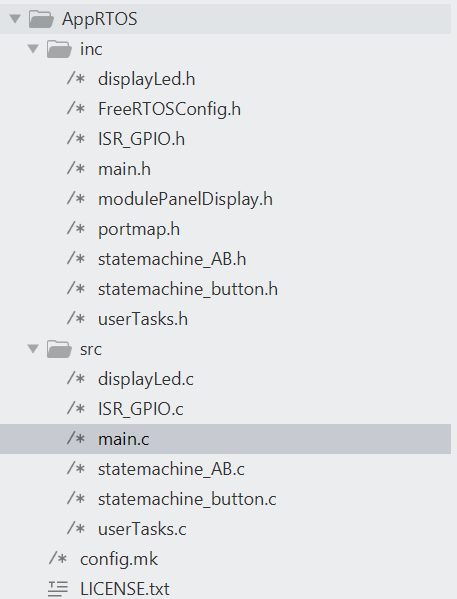
\includegraphics[width=1\textwidth]{./Figures/estructuraCodigos.png}
	\caption{Estructura del código en C.}
	\label{fig:codestructure}
\end{figure}

\begin{figure}[ht]
	\centering
	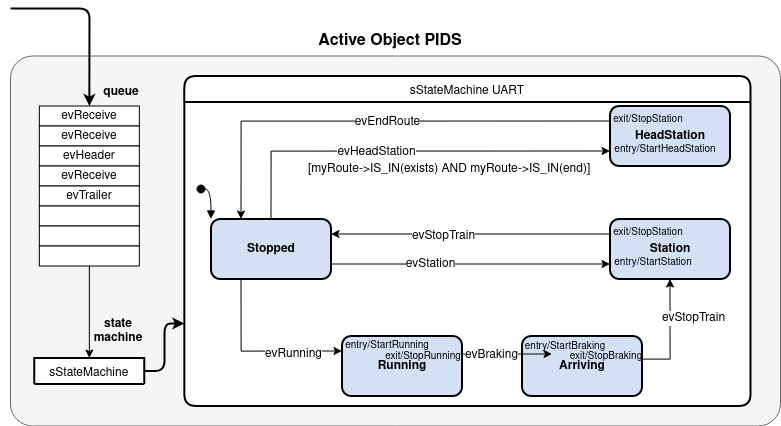
\includegraphics[width=1\textwidth]{./Figures/fsmTrain.png}
	\caption{Diagrama del objeto activo PIDS y detalle de la máquina de estados asociada.}
	\label{fig:fsmTrain}
\end{figure}

\pagebreak
\section{Firmware}


\begin{figure}[ht]
	\centering
	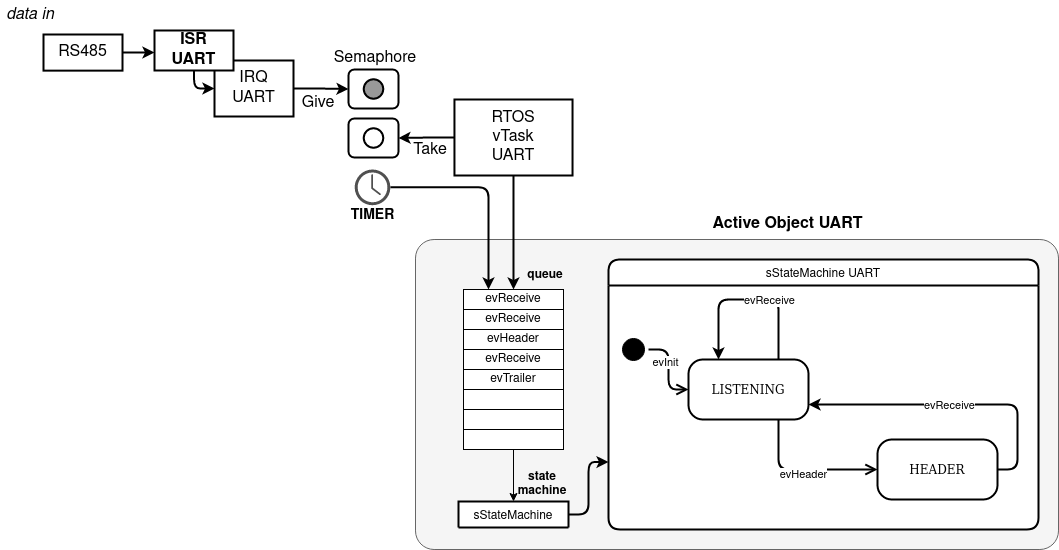
\includegraphics[width=1\textwidth]{./Figures/fsmUART.png}
	\caption{Diagrama de detalle de la implementación en RTOS del objeto activo UART.}
	\label{fig:fsmUART}
\end{figure}


\begin{figure}[ht]
	\centering
	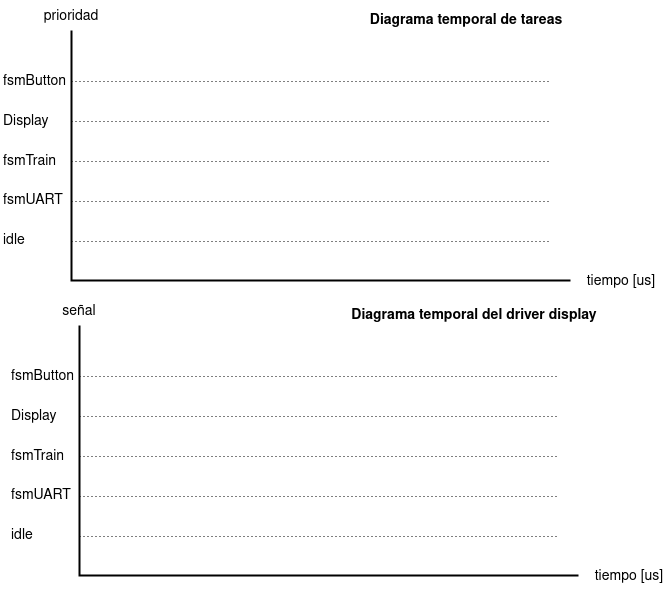
\includegraphics[width=1\textwidth]{./Figures/diagramasTemporales.png}
	\caption{}
	\label{fig:diagramasTemporales}
\end{figure}

\pagebreak
\section{Hardware}

\begin{figure}[ht]
	\centering
	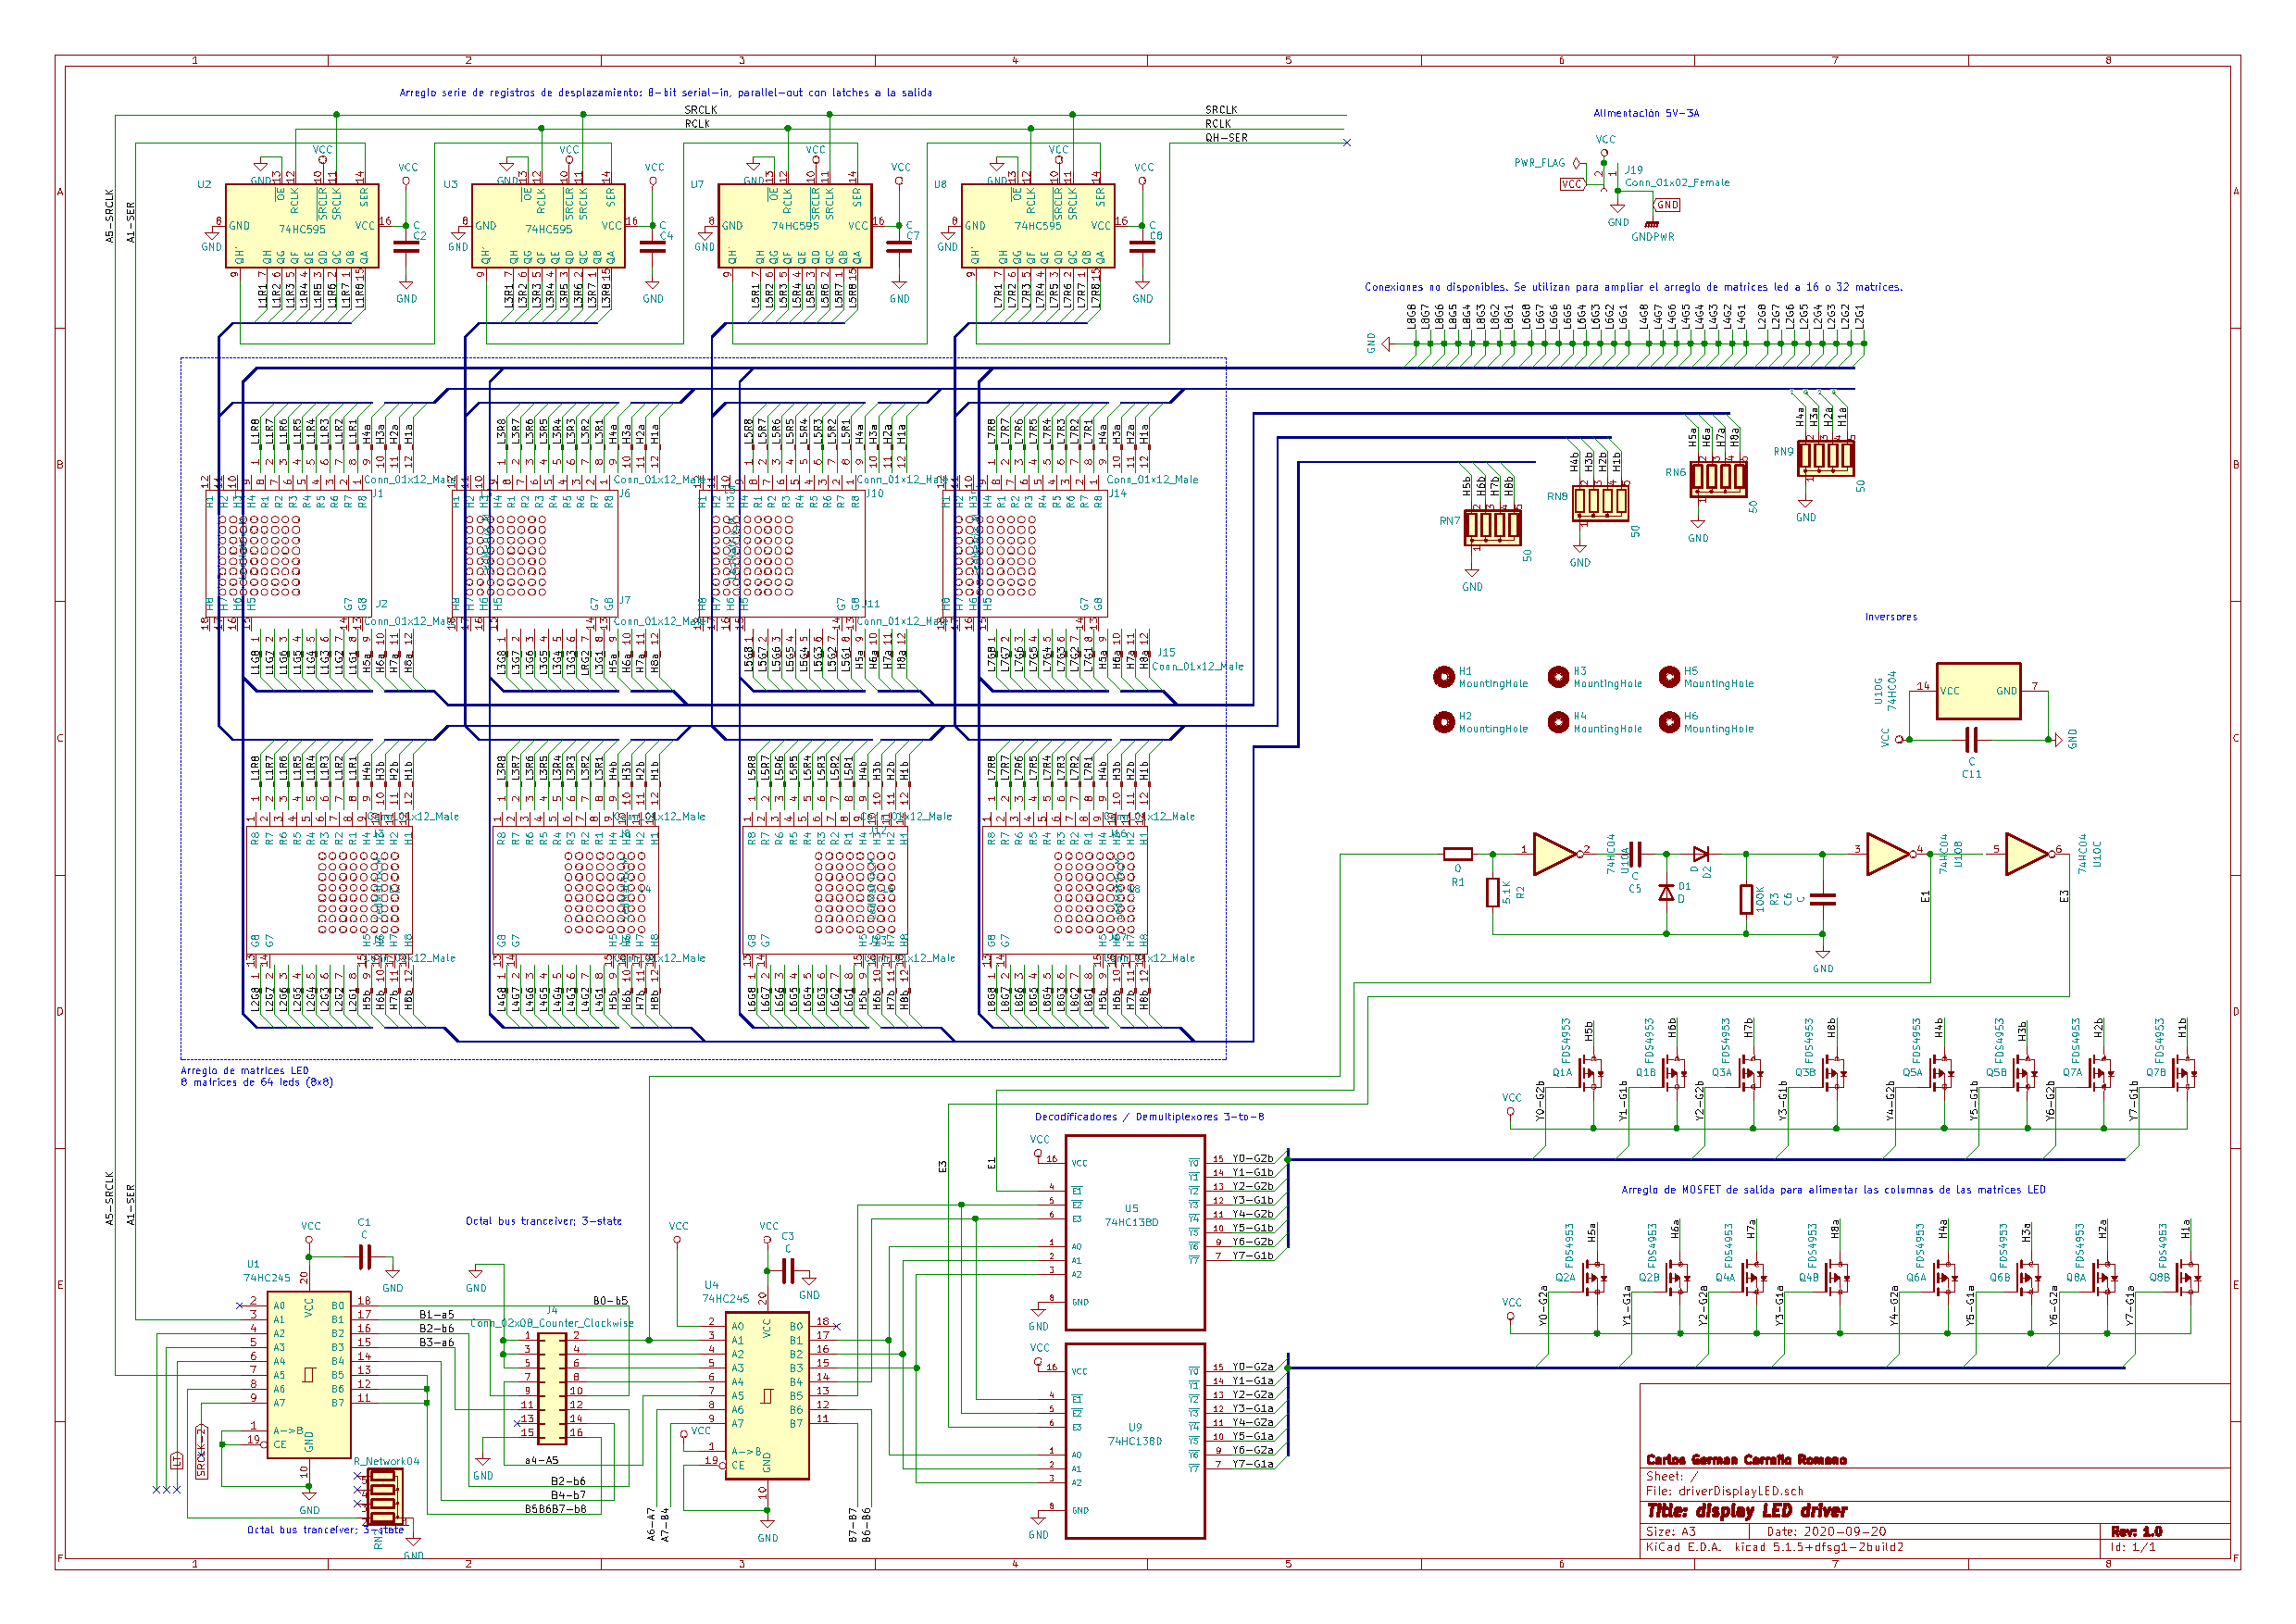
\includegraphics[width=1\textwidth]{./Figures/output.driverLED.pdf}
	\caption{Circuito esquemático de la placa driver de los carteles de matriz LED.}
	\label{fig:schDriverLED}
\end{figure}

\begin{figure}[ht]
	\centering
	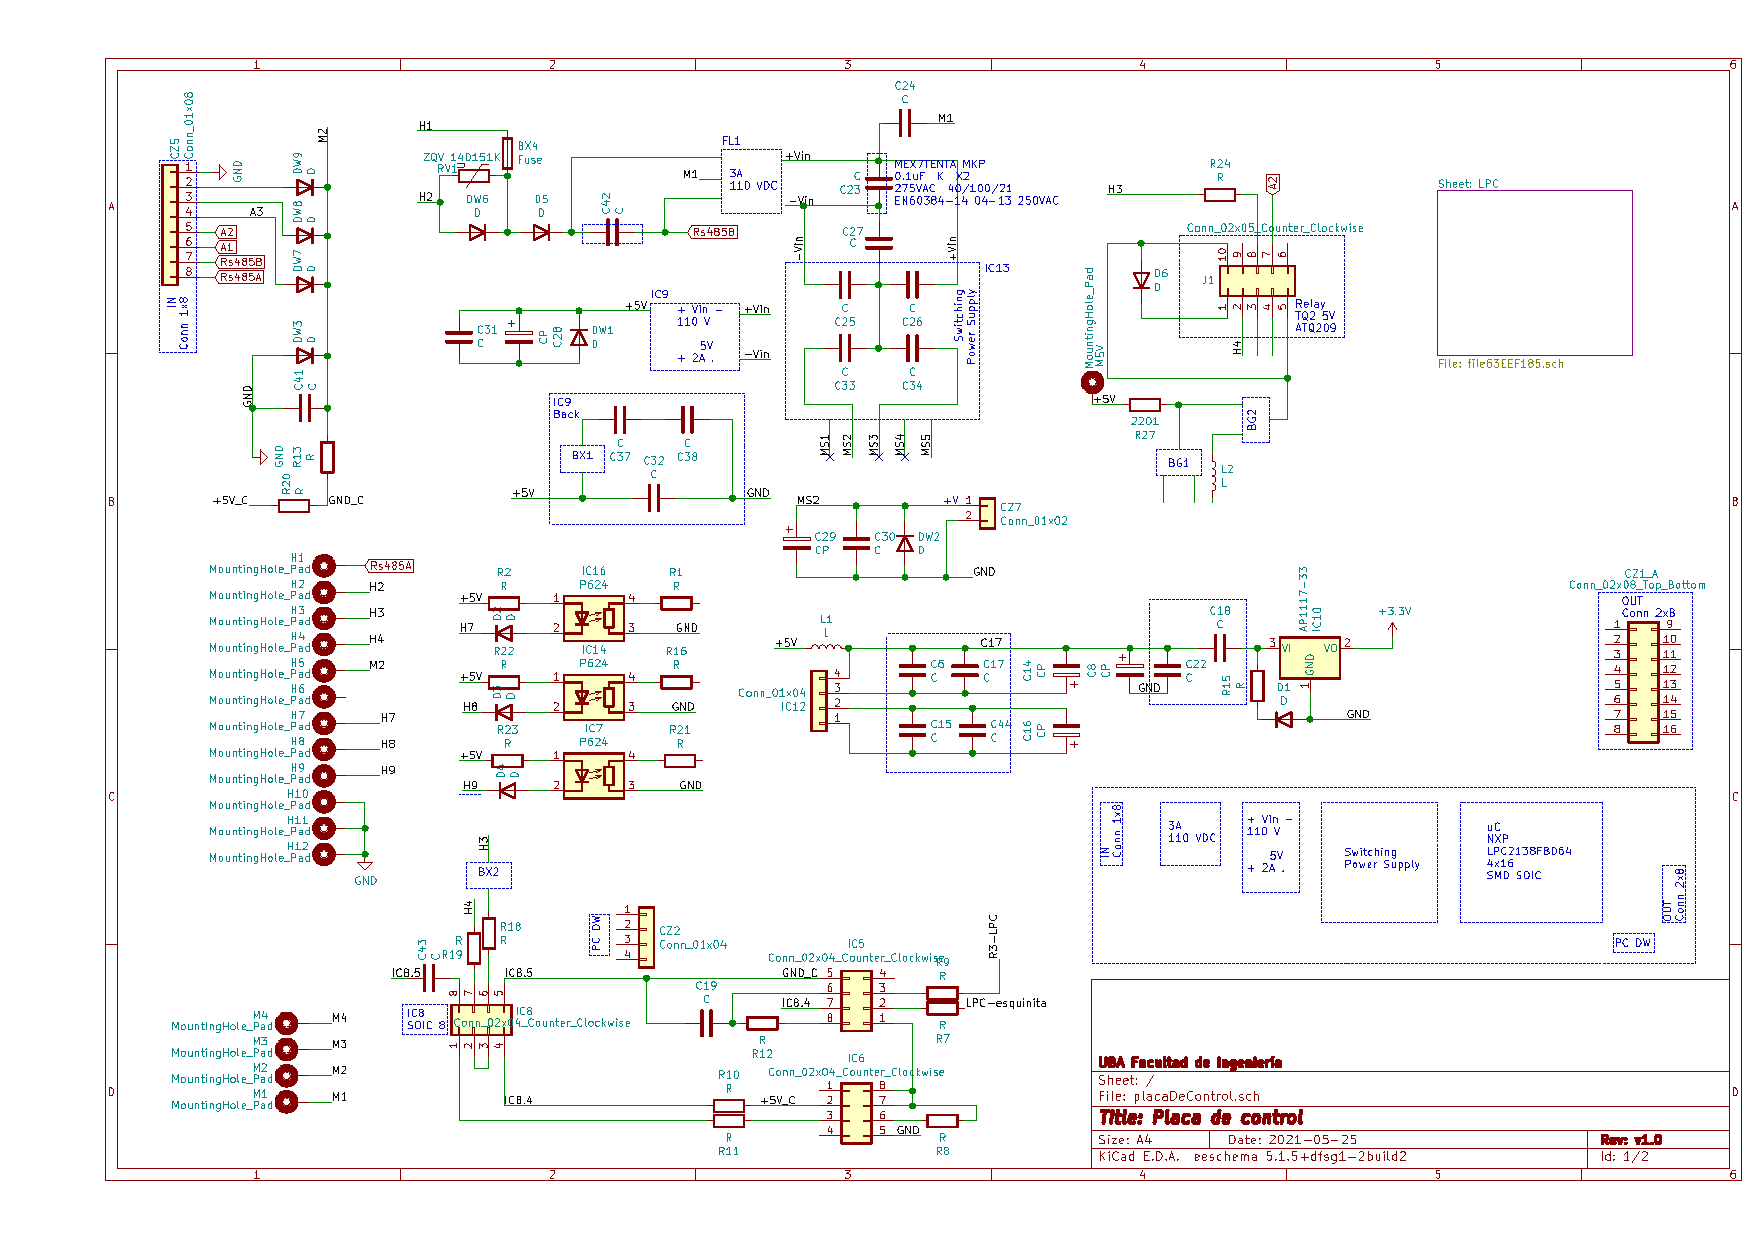
\includegraphics[width=1\textwidth]{./Figures/output.placaControl.pdf}
	\caption{Circuito esquemático de la placa de control de los carteles LED de salón.}
	\label{fig:schController}
\end{figure}